% **************************************************************************************************************
% A Classic Thesis Style
% An Homage to The Elements of Typographic Style
%
% Copyright (C) 2015 André Miede http://www.miede.de
%
% If you like the style then I would appreciate a postcard. My address 
% can be found in the file ClassicThesis.pdf. A collection of the 
% postcards I received so far is available online at 
% http://postcards.miede.de
%
% License:
% This program is free software; you can redistribute it and/or modify
% it under the terms of the GNU General Public License as published by
% the Free Software Foundation; either version 2 of the License, or
% (at your option) any later version.
%
% This program is distributed in the hope that it will be useful,
% but WITHOUT ANY WARRANTY; without even the implied warranty of
% MERCHANTABILITY or FITNESS FOR A PARTICULAR PURPOSE.  See the
% GNU General Public License for more details.
%
% You should have received a copy of the GNU General Public License
% along with this program; see the file COPYING.  If not, write to
% the Free Software Foundation, Inc., 59 Temple Place - Suite 330,
% Boston, MA 02111-1307, USA.
%
% **************************************************************************************************************
\RequirePackage{fix-cm} % fix some latex issues see: http://texdoc.net/texmf-dist/doc/latex/base/fixltx2e.pdf
\documentclass[ oneside,openright,titlepage,numbers=noenddot,headinclude,%1headlines,% letterpaper a4paper
                footinclude=true,cleardoublepage=empty,abstractoff, % <--- obsolete, remove (todo)
                BCOR=5mm,paper=a4,fontsize=11pt,%11pt,a4paper,%
                ngerman,american,%
                ]{scrreprt}

%********************************************************************
% Note: Make all your adjustments in here
%*******************************************************
% ****************************************************************************************************
% classicthesis-config.tex 
% formerly known as loadpackages.sty, classicthesis-ldpkg.sty, and classicthesis-preamble.sty 
% Use it at the beginning of your ClassicThesis.tex, or as a LaTeX Preamble 
% in your ClassicThesis.{tex,lyx} with % ****************************************************************************************************
% classicthesis-config.tex 
% formerly known as loadpackages.sty, classicthesis-ldpkg.sty, and classicthesis-preamble.sty 
% Use it at the beginning of your ClassicThesis.tex, or as a LaTeX Preamble 
% in your ClassicThesis.{tex,lyx} with % ****************************************************************************************************
% classicthesis-config.tex 
% formerly known as loadpackages.sty, classicthesis-ldpkg.sty, and classicthesis-preamble.sty 
% Use it at the beginning of your ClassicThesis.tex, or as a LaTeX Preamble 
% in your ClassicThesis.{tex,lyx} with \input{classicthesis-config}
% ****************************************************************************************************  
% If you like the classicthesis, then I would appreciate a postcard. 
% My address can be found in the file ClassicThesis.pdf. A collection 
% of the postcards I received so far is available online at 
% http://postcards.miede.de
% ****************************************************************************************************


% ****************************************************************************************************
% 0. Set the encoding of your files. UTF-8 is the only sensible encoding nowadays. If you can't read
% äöüßáéçèê∂åëæƒÏ€ then change the encoding setting in your editor, not the line below. If your editor
% does not support utf8 use another editor!
% ****************************************************************************************************
\PassOptionsToPackage{utf8}{inputenc}
	\usepackage{inputenc}

% ****************************************************************************************************
% 1. Configure classicthesis for your needs here, e.g., remove "drafting" below 
% in order to deactivate the time-stamp on the pages
% ****************************************************************************************************
\PassOptionsToPackage{eulerchapternumbers,listings,%drafting,
					 pdfspacing,%floatperchapter,%linedheaders,%
					 subfig,beramono,eulermath,parts}{classicthesis}                                        
% ********************************************************************
% Available options for classicthesis.sty 
% (see ClassicThesis.pdf for more information):
% drafting
% parts nochapters linedheaders
% eulerchapternumbers beramono eulermath pdfspacing minionprospacing
% tocaligned dottedtoc manychapters
% listings floatperchapter subfig
% ********************************************************************


% ****************************************************************************************************
% 2. Personal data and user ad-hoc commands
% ****************************************************************************************************
\input{info}

% ********************************************************************
% Setup, finetuning, and useful commands
% ********************************************************************
\newcounter{dummy} % necessary for correct hyperlinks (to index, bib, etc.)
\newlength{\abcd} % for ab..z string length calculation
\providecommand{\mLyX}{L\kern-.1667em\lower.25em\hbox{Y}\kern-.125emX\@}
\newcommand{\ie}{i.\,e.}
\newcommand{\Ie}{I.\,e.}
\newcommand{\eg}{e.\,g.}
\newcommand{\Eg}{E.\,g.} 
% ****************************************************************************************************


% ****************************************************************************************************
% 3. Loading some handy packages
% ****************************************************************************************************
% ******************************************************************** 
% Packages with options that might require adjustments
% ******************************************************************** 
%\PassOptionsToPackage{ngerman,american}{babel}   % change this to your language(s)
% Spanish languages need extra options in order to work with this template
%\PassOptionsToPackage{spanish,es-lcroman}{babel}
	\usepackage{babel}                  

\usepackage{csquotes}
%\PassOptionsToPackage{%
%    backend=biber, %instead of bibtex
%	backend=bibtex8,bibencoding=ascii,%
%	language=auto,%
%    style=lnig,
%	%style=numeric-comp,%
%    %style=authoryear-comp, % Author 1999, 2010
%    %bibstyle=authoryear,dashed=false, % dashed: substitute rep. author with ---
%    sorting=nyt, % name, year, title
%    maxbibnames=10, % default: 3, et al.
%    %backref=true,%
%    natbib=true % natbib compatibility mode (\citep and \citet still work)
%}{biblatex}
%    \usepackage{biblatex}
% bibliography

\PassOptionsToPackage{fleqn}{amsmath}       % math environments and more by the AMS 
    \usepackage{amsmath}

% ******************************************************************** 
% General useful packages
% ******************************************************************** 
\PassOptionsToPackage{T1}{fontenc} % T2A for cyrillics
    \usepackage{fontenc}     
\usepackage{textcomp} % fix warning with missing font shapes
\usepackage{scrhack} % fix warnings when using KOMA with listings package          
\usepackage{xspace} % to get the spacing after macros right  
\usepackage{mparhack} % get marginpar right
\usepackage{fixltx2e} % fixes some LaTeX stuff --> since 2015 in the LaTeX kernel (see below)
%\usepackage[latest]{latexrelease} % will be used once available in more distributions (ISSUE #107)
\PassOptionsToPackage{printonlyused,smaller}{acronym} 
    \usepackage{acronym} % nice macros for handling all acronyms in the thesis
    %\renewcommand{\bflabel}[1]{{#1}\hfill} % fix the list of acronyms --> no longer working
    %\renewcommand*{\acsfont}[1]{\textsc{#1}} 
    \renewcommand*{\aclabelfont}[1]{\acsfont{#1}}
% ****************************************************************************************************


% ****************************************************************************************************
% 4. Setup floats: tables, (sub)figures, and captions
% ****************************************************************************************************
\usepackage{tabularx} % better tables
    \setlength{\extrarowheight}{3pt} % increase table row height
\newcommand{\tableheadline}[1]{\multicolumn{1}{c}{\spacedlowsmallcaps{#1}}}
\newcommand{\myfloatalign}{\centering} % to be used with each float for alignment
\usepackage{caption}
% Thanks to cgnieder and Claus Lahiri
% http://tex.stackexchange.com/questions/69349/spacedlowsmallcaps-in-caption-label
% [REMOVED DUE TO OTHER PROBLEMS, SEE ISSUE #82]    
%\DeclareCaptionLabelFormat{smallcaps}{\bothIfFirst{#1}{~}\MakeTextLowercase{\textsc{#2}}}
%\captionsetup{font=small,labelformat=smallcaps} % format=hang,
\captionsetup{font=small} % format=hang,
\usepackage{subfig}  
% ****************************************************************************************************


% ****************************************************************************************************
% 5. Setup code listings
% ****************************************************************************************************
\usepackage{listings} 
%\lstset{emph={trueIndex,root},emphstyle=\color{BlueViolet}}%\underbar} % for special keywords
\lstset{language=[LaTeX]Tex,%C++,
    morekeywords={PassOptionsToPackage,selectlanguage},
    keywordstyle=\color{RoyalBlue},%\bfseries,
    basicstyle=\small\ttfamily,
    %identifierstyle=\color{NavyBlue},
    commentstyle=\color{Green}\ttfamily,
    stringstyle=\rmfamily,
    numbers=none,%left,%
    numberstyle=\scriptsize,%\tiny
    stepnumber=5,
    numbersep=8pt,
    showstringspaces=false,
    breaklines=true,
    %frameround=ftff,
    %frame=single,
    belowcaptionskip=.75\baselineskip
    %frame=L
} 
% ****************************************************************************************************             


% ****************************************************************************************************
% 6. PDFLaTeX, hyperreferences and citation backreferences
% ****************************************************************************************************
% ********************************************************************
% Using PDFLaTeX
% ********************************************************************
\PassOptionsToPackage{pdftex,hyperfootnotes=false,pdfpagelabels}{hyperref}
    \usepackage{hyperref}  % backref linktocpage pagebackref
\pdfcompresslevel=9
\pdfadjustspacing=1 
\PassOptionsToPackage{pdftex}{graphicx}
    \usepackage{graphicx} 
 

% ********************************************************************
% Hyperreferences
% ********************************************************************
\hypersetup{%
    %draft, % = no hyperlinking at all (useful in b/w printouts)
    %colorlinks=true, linktocpage=true, pdfstartpage=3, pdfstartview=FitV,%
    % uncomment the following line if you want to have black links (e.g., for printing)
    colorlinks=false, linktocpage=false, pdfstartpage=3, pdfstartview=FitV, pdfborder={0 0 0},%
    breaklinks=true, pdfpagemode=UseNone, pageanchor=true, pdfpagemode=UseOutlines,%
    plainpages=false, bookmarksnumbered, bookmarksopen=true, bookmarksopenlevel=1,%
    hypertexnames=true, pdfhighlight=/O,%nesting=true,%frenchlinks,%
    urlcolor=webbrown, linkcolor=RoyalBlue, citecolor=webgreen, %pagecolor=RoyalBlue,%
    %urlcolor=Black, linkcolor=Black, citecolor=Black, %pagecolor=Black,%
    pdftitle={\myTitle},%
    pdfauthor={\textcopyright\ \myName, \myUni},%
    pdfsubject={},%
    pdfkeywords={},%
    pdfcreator={pdfLaTeX},%
    pdfproducer={LaTeX with hyperref and classicthesis}%
}   

% ********************************************************************
% Setup autoreferences
% ********************************************************************
% There are some issues regarding autorefnames
% http://www.ureader.de/msg/136221647.aspx
% http://www.tex.ac.uk/cgi-bin/texfaq2html?label=latexwords
% you have to redefine the makros for the 
% language you use, e.g., american, ngerman
% (as chosen when loading babel/AtBeginDocument)
% ********************************************************************
\makeatletter
\@ifpackageloaded{babel}%
    {%
       \addto\extrasamerican{%
			\renewcommand*{\figureautorefname}{Figure}%
			\renewcommand*{\tableautorefname}{Table}%
			\renewcommand*{\partautorefname}{Part}%
			\renewcommand*{\chapterautorefname}{Chapter}%
			\renewcommand*{\sectionautorefname}{Section}%
			\renewcommand*{\subsectionautorefname}{Section}%
			\renewcommand*{\subsubsectionautorefname}{Section}%     
                }%
       \addto\extrasngerman{% 
			\renewcommand*{\paragraphautorefname}{Absatz}%
			\renewcommand*{\subparagraphautorefname}{Unterabsatz}%
			\renewcommand*{\footnoteautorefname}{Fu\"snote}%
			\renewcommand*{\FancyVerbLineautorefname}{Zeile}%
			\renewcommand*{\theoremautorefname}{Theorem}%
			\renewcommand*{\appendixautorefname}{Anhang}%
			\renewcommand*{\equationautorefname}{Gleichung}%        
			\renewcommand*{\itemautorefname}{Punkt}%
                }%  
            % Fix to getting autorefs for subfigures right (thanks to Belinda Vogt for changing the definition)
            \providecommand{\subfigureautorefname}{\figureautorefname}%             
    }{\relax}
\makeatother


% ****************************************************************************************************
% 7. Last calls before the bar closes
% ****************************************************************************************************
% ********************************************************************
% Development Stuff
% ********************************************************************
\listfiles
%\PassOptionsToPackage{l2tabu,orthodox,abort}{nag}
%   \usepackage{nag}
%\PassOptionsToPackage{warning, all}{onlyamsmath}
%   \usepackage{onlyamsmath}

% ********************************************************************
% Last, but not least...
% ********************************************************************
\usepackage[dottedtoc]{classicthesis} 


%For the colored backgrounds
\usepackage{xcolor}
\definecolor{grau}{gray}{.85}	
\definecolor{grau2}{gray}{.95}
% ****************************************************************************************************


% ****************************************************************************************************
% 8. Further adjustments (experimental)
% ****************************************************************************************************
% ********************************************************************
% Changing the text area
% ********************************************************************
%\linespread{1.05} % a bit more for Palatino
\areaset[current]{412pt}{761pt} % 686 (factor 2.2) + 33 head + 42 head \the\footskip
%\setlength{\marginparwidth}{7em}%
%\setlength{\marginparsep}{2em}%

% ********************************************************************
% Using different fonts
% ********************************************************************
%\usepackage[oldstylenums]{kpfonts} % oldstyle notextcomp
%\usepackage[osf]{libertine}
%\usepackage[light,condensed,math]{iwona}
%\renewcommand{\sfdefault}{iwona}
%\usepackage{lmodern} % <-- no osf support :-(
%\usepackage{cfr-lm} % 
%\usepackage[urw-garamond]{mathdesign} <-- no osf support :-(
%\usepackage[default,osfigures]{opensans} % scale=0.95 
%\usepackage[sfdefault]{FiraSans}
% ****************************************************************************************************

% ****************************************************************************************************  
% If you like the classicthesis, then I would appreciate a postcard. 
% My address can be found in the file ClassicThesis.pdf. A collection 
% of the postcards I received so far is available online at 
% http://postcards.miede.de
% ****************************************************************************************************


% ****************************************************************************************************
% 0. Set the encoding of your files. UTF-8 is the only sensible encoding nowadays. If you can't read
% äöüßáéçèê∂åëæƒÏ€ then change the encoding setting in your editor, not the line below. If your editor
% does not support utf8 use another editor!
% ****************************************************************************************************
\PassOptionsToPackage{utf8}{inputenc}
	\usepackage{inputenc}

% ****************************************************************************************************
% 1. Configure classicthesis for your needs here, e.g., remove "drafting" below 
% in order to deactivate the time-stamp on the pages
% ****************************************************************************************************
\PassOptionsToPackage{eulerchapternumbers,listings,%drafting,
					 pdfspacing,%floatperchapter,%linedheaders,%
					 subfig,beramono,eulermath,parts}{classicthesis}                                        
% ********************************************************************
% Available options for classicthesis.sty 
% (see ClassicThesis.pdf for more information):
% drafting
% parts nochapters linedheaders
% eulerchapternumbers beramono eulermath pdfspacing minionprospacing
% tocaligned dottedtoc manychapters
% listings floatperchapter subfig
% ********************************************************************


% ****************************************************************************************************
% 2. Personal data and user ad-hoc commands
% ****************************************************************************************************
\def\myLanguage{de} % de, en
\newcommand{\myTitle}{3D-Spieleentwicklung mit Java\xspace}
\newcommand{\myTypeOfWork}{Seminararbeit\xspace}
\newcommand{\myName}{Julian Wadephul und Florian Rottach\xspace}
\newcommand{\myProf}{Prof.~Dr.~Vorname Nachname\xspace}
\newcommand{\myCourse}{Wirtschaftsingenieurwesen}
\newcommand{\mySupervisor}{Jonas Lehner\xspace}
\newcommand{\myInstitute}{Institut für Angewandte Informatik und Formale Beschreibungsverfahren\xspace}
\newcommand{\myDepartment}{KIT-Fakultät für Wirtschaftswissenschaften\xspace}
\newcommand{\myUni}{KIT - Die Forschungsuniversität in der Helmholtz-Gemeinschaft\xspace}
\newcommand{\myLocation}{Karlsruhe\xspace}
\newcommand{\myTime}{20. Februar 2017\xspace}

% ********************************************************************
% Setup, finetuning, and useful commands
% ********************************************************************
\newcounter{dummy} % necessary for correct hyperlinks (to index, bib, etc.)
\newlength{\abcd} % for ab..z string length calculation
\providecommand{\mLyX}{L\kern-.1667em\lower.25em\hbox{Y}\kern-.125emX\@}
\newcommand{\ie}{i.\,e.}
\newcommand{\Ie}{I.\,e.}
\newcommand{\eg}{e.\,g.}
\newcommand{\Eg}{E.\,g.} 
% ****************************************************************************************************


% ****************************************************************************************************
% 3. Loading some handy packages
% ****************************************************************************************************
% ******************************************************************** 
% Packages with options that might require adjustments
% ******************************************************************** 
%\PassOptionsToPackage{ngerman,american}{babel}   % change this to your language(s)
% Spanish languages need extra options in order to work with this template
%\PassOptionsToPackage{spanish,es-lcroman}{babel}
	\usepackage{babel}                  

\usepackage{csquotes}
%\PassOptionsToPackage{%
%    backend=biber, %instead of bibtex
%	backend=bibtex8,bibencoding=ascii,%
%	language=auto,%
%    style=lnig,
%	%style=numeric-comp,%
%    %style=authoryear-comp, % Author 1999, 2010
%    %bibstyle=authoryear,dashed=false, % dashed: substitute rep. author with ---
%    sorting=nyt, % name, year, title
%    maxbibnames=10, % default: 3, et al.
%    %backref=true,%
%    natbib=true % natbib compatibility mode (\citep and \citet still work)
%}{biblatex}
%    \usepackage{biblatex}
% bibliography

\PassOptionsToPackage{fleqn}{amsmath}       % math environments and more by the AMS 
    \usepackage{amsmath}

% ******************************************************************** 
% General useful packages
% ******************************************************************** 
\PassOptionsToPackage{T1}{fontenc} % T2A for cyrillics
    \usepackage{fontenc}     
\usepackage{textcomp} % fix warning with missing font shapes
\usepackage{scrhack} % fix warnings when using KOMA with listings package          
\usepackage{xspace} % to get the spacing after macros right  
\usepackage{mparhack} % get marginpar right
\usepackage{fixltx2e} % fixes some LaTeX stuff --> since 2015 in the LaTeX kernel (see below)
%\usepackage[latest]{latexrelease} % will be used once available in more distributions (ISSUE #107)
\PassOptionsToPackage{printonlyused,smaller}{acronym} 
    \usepackage{acronym} % nice macros for handling all acronyms in the thesis
    %\renewcommand{\bflabel}[1]{{#1}\hfill} % fix the list of acronyms --> no longer working
    %\renewcommand*{\acsfont}[1]{\textsc{#1}} 
    \renewcommand*{\aclabelfont}[1]{\acsfont{#1}}
% ****************************************************************************************************


% ****************************************************************************************************
% 4. Setup floats: tables, (sub)figures, and captions
% ****************************************************************************************************
\usepackage{tabularx} % better tables
    \setlength{\extrarowheight}{3pt} % increase table row height
\newcommand{\tableheadline}[1]{\multicolumn{1}{c}{\spacedlowsmallcaps{#1}}}
\newcommand{\myfloatalign}{\centering} % to be used with each float for alignment
\usepackage{caption}
% Thanks to cgnieder and Claus Lahiri
% http://tex.stackexchange.com/questions/69349/spacedlowsmallcaps-in-caption-label
% [REMOVED DUE TO OTHER PROBLEMS, SEE ISSUE #82]    
%\DeclareCaptionLabelFormat{smallcaps}{\bothIfFirst{#1}{~}\MakeTextLowercase{\textsc{#2}}}
%\captionsetup{font=small,labelformat=smallcaps} % format=hang,
\captionsetup{font=small} % format=hang,
\usepackage{subfig}  
% ****************************************************************************************************


% ****************************************************************************************************
% 5. Setup code listings
% ****************************************************************************************************
\usepackage{listings} 
%\lstset{emph={trueIndex,root},emphstyle=\color{BlueViolet}}%\underbar} % for special keywords
\lstset{language=[LaTeX]Tex,%C++,
    morekeywords={PassOptionsToPackage,selectlanguage},
    keywordstyle=\color{RoyalBlue},%\bfseries,
    basicstyle=\small\ttfamily,
    %identifierstyle=\color{NavyBlue},
    commentstyle=\color{Green}\ttfamily,
    stringstyle=\rmfamily,
    numbers=none,%left,%
    numberstyle=\scriptsize,%\tiny
    stepnumber=5,
    numbersep=8pt,
    showstringspaces=false,
    breaklines=true,
    %frameround=ftff,
    %frame=single,
    belowcaptionskip=.75\baselineskip
    %frame=L
} 
% ****************************************************************************************************             


% ****************************************************************************************************
% 6. PDFLaTeX, hyperreferences and citation backreferences
% ****************************************************************************************************
% ********************************************************************
% Using PDFLaTeX
% ********************************************************************
\PassOptionsToPackage{pdftex,hyperfootnotes=false,pdfpagelabels}{hyperref}
    \usepackage{hyperref}  % backref linktocpage pagebackref
\pdfcompresslevel=9
\pdfadjustspacing=1 
\PassOptionsToPackage{pdftex}{graphicx}
    \usepackage{graphicx} 
 

% ********************************************************************
% Hyperreferences
% ********************************************************************
\hypersetup{%
    %draft, % = no hyperlinking at all (useful in b/w printouts)
    %colorlinks=true, linktocpage=true, pdfstartpage=3, pdfstartview=FitV,%
    % uncomment the following line if you want to have black links (e.g., for printing)
    colorlinks=false, linktocpage=false, pdfstartpage=3, pdfstartview=FitV, pdfborder={0 0 0},%
    breaklinks=true, pdfpagemode=UseNone, pageanchor=true, pdfpagemode=UseOutlines,%
    plainpages=false, bookmarksnumbered, bookmarksopen=true, bookmarksopenlevel=1,%
    hypertexnames=true, pdfhighlight=/O,%nesting=true,%frenchlinks,%
    urlcolor=webbrown, linkcolor=RoyalBlue, citecolor=webgreen, %pagecolor=RoyalBlue,%
    %urlcolor=Black, linkcolor=Black, citecolor=Black, %pagecolor=Black,%
    pdftitle={\myTitle},%
    pdfauthor={\textcopyright\ \myName, \myUni},%
    pdfsubject={},%
    pdfkeywords={},%
    pdfcreator={pdfLaTeX},%
    pdfproducer={LaTeX with hyperref and classicthesis}%
}   

% ********************************************************************
% Setup autoreferences
% ********************************************************************
% There are some issues regarding autorefnames
% http://www.ureader.de/msg/136221647.aspx
% http://www.tex.ac.uk/cgi-bin/texfaq2html?label=latexwords
% you have to redefine the makros for the 
% language you use, e.g., american, ngerman
% (as chosen when loading babel/AtBeginDocument)
% ********************************************************************
\makeatletter
\@ifpackageloaded{babel}%
    {%
       \addto\extrasamerican{%
			\renewcommand*{\figureautorefname}{Figure}%
			\renewcommand*{\tableautorefname}{Table}%
			\renewcommand*{\partautorefname}{Part}%
			\renewcommand*{\chapterautorefname}{Chapter}%
			\renewcommand*{\sectionautorefname}{Section}%
			\renewcommand*{\subsectionautorefname}{Section}%
			\renewcommand*{\subsubsectionautorefname}{Section}%     
                }%
       \addto\extrasngerman{% 
			\renewcommand*{\paragraphautorefname}{Absatz}%
			\renewcommand*{\subparagraphautorefname}{Unterabsatz}%
			\renewcommand*{\footnoteautorefname}{Fu\"snote}%
			\renewcommand*{\FancyVerbLineautorefname}{Zeile}%
			\renewcommand*{\theoremautorefname}{Theorem}%
			\renewcommand*{\appendixautorefname}{Anhang}%
			\renewcommand*{\equationautorefname}{Gleichung}%        
			\renewcommand*{\itemautorefname}{Punkt}%
                }%  
            % Fix to getting autorefs for subfigures right (thanks to Belinda Vogt for changing the definition)
            \providecommand{\subfigureautorefname}{\figureautorefname}%             
    }{\relax}
\makeatother


% ****************************************************************************************************
% 7. Last calls before the bar closes
% ****************************************************************************************************
% ********************************************************************
% Development Stuff
% ********************************************************************
\listfiles
%\PassOptionsToPackage{l2tabu,orthodox,abort}{nag}
%   \usepackage{nag}
%\PassOptionsToPackage{warning, all}{onlyamsmath}
%   \usepackage{onlyamsmath}

% ********************************************************************
% Last, but not least...
% ********************************************************************
\usepackage[dottedtoc]{classicthesis} 


%For the colored backgrounds
\usepackage{xcolor}
\definecolor{grau}{gray}{.85}	
\definecolor{grau2}{gray}{.95}
% ****************************************************************************************************


% ****************************************************************************************************
% 8. Further adjustments (experimental)
% ****************************************************************************************************
% ********************************************************************
% Changing the text area
% ********************************************************************
%\linespread{1.05} % a bit more for Palatino
\areaset[current]{412pt}{761pt} % 686 (factor 2.2) + 33 head + 42 head \the\footskip
%\setlength{\marginparwidth}{7em}%
%\setlength{\marginparsep}{2em}%

% ********************************************************************
% Using different fonts
% ********************************************************************
%\usepackage[oldstylenums]{kpfonts} % oldstyle notextcomp
%\usepackage[osf]{libertine}
%\usepackage[light,condensed,math]{iwona}
%\renewcommand{\sfdefault}{iwona}
%\usepackage{lmodern} % <-- no osf support :-(
%\usepackage{cfr-lm} % 
%\usepackage[urw-garamond]{mathdesign} <-- no osf support :-(
%\usepackage[default,osfigures]{opensans} % scale=0.95 
%\usepackage[sfdefault]{FiraSans}
% ****************************************************************************************************

% ****************************************************************************************************  
% If you like the classicthesis, then I would appreciate a postcard. 
% My address can be found in the file ClassicThesis.pdf. A collection 
% of the postcards I received so far is available online at 
% http://postcards.miede.de
% ****************************************************************************************************


% ****************************************************************************************************
% 0. Set the encoding of your files. UTF-8 is the only sensible encoding nowadays. If you can't read
% äöüßáéçèê∂åëæƒÏ€ then change the encoding setting in your editor, not the line below. If your editor
% does not support utf8 use another editor!
% ****************************************************************************************************
\PassOptionsToPackage{utf8}{inputenc}
	\usepackage{inputenc}

% ****************************************************************************************************
% 1. Configure classicthesis for your needs here, e.g., remove "drafting" below 
% in order to deactivate the time-stamp on the pages
% ****************************************************************************************************
\PassOptionsToPackage{eulerchapternumbers,listings,%drafting,
					 pdfspacing,%floatperchapter,%linedheaders,%
					 subfig,beramono,eulermath,parts}{classicthesis}                                        
% ********************************************************************
% Available options for classicthesis.sty 
% (see ClassicThesis.pdf for more information):
% drafting
% parts nochapters linedheaders
% eulerchapternumbers beramono eulermath pdfspacing minionprospacing
% tocaligned dottedtoc manychapters
% listings floatperchapter subfig
% ********************************************************************


% ****************************************************************************************************
% 2. Personal data and user ad-hoc commands
% ****************************************************************************************************
\def\myLanguage{de} % de, en
\newcommand{\myTitle}{3D-Spieleentwicklung mit Java\xspace}
\newcommand{\myTypeOfWork}{Seminararbeit\xspace}
\newcommand{\myName}{Julian Wadephul und Florian Rottach\xspace}
\newcommand{\myProf}{Prof.~Dr.~Vorname Nachname\xspace}
\newcommand{\myCourse}{Wirtschaftsingenieurwesen}
\newcommand{\mySupervisor}{Jonas Lehner\xspace}
\newcommand{\myInstitute}{Institut für Angewandte Informatik und Formale Beschreibungsverfahren\xspace}
\newcommand{\myDepartment}{KIT-Fakultät für Wirtschaftswissenschaften\xspace}
\newcommand{\myUni}{KIT - Die Forschungsuniversität in der Helmholtz-Gemeinschaft\xspace}
\newcommand{\myLocation}{Karlsruhe\xspace}
\newcommand{\myTime}{20. Februar 2017\xspace}

% ********************************************************************
% Setup, finetuning, and useful commands
% ********************************************************************
\newcounter{dummy} % necessary for correct hyperlinks (to index, bib, etc.)
\newlength{\abcd} % for ab..z string length calculation
\providecommand{\mLyX}{L\kern-.1667em\lower.25em\hbox{Y}\kern-.125emX\@}
\newcommand{\ie}{i.\,e.}
\newcommand{\Ie}{I.\,e.}
\newcommand{\eg}{e.\,g.}
\newcommand{\Eg}{E.\,g.} 
% ****************************************************************************************************


% ****************************************************************************************************
% 3. Loading some handy packages
% ****************************************************************************************************
% ******************************************************************** 
% Packages with options that might require adjustments
% ******************************************************************** 
%\PassOptionsToPackage{ngerman,american}{babel}   % change this to your language(s)
% Spanish languages need extra options in order to work with this template
%\PassOptionsToPackage{spanish,es-lcroman}{babel}
	\usepackage{babel}                  

\usepackage{csquotes}
%\PassOptionsToPackage{%
%    backend=biber, %instead of bibtex
%	backend=bibtex8,bibencoding=ascii,%
%	language=auto,%
%    style=lnig,
%	%style=numeric-comp,%
%    %style=authoryear-comp, % Author 1999, 2010
%    %bibstyle=authoryear,dashed=false, % dashed: substitute rep. author with ---
%    sorting=nyt, % name, year, title
%    maxbibnames=10, % default: 3, et al.
%    %backref=true,%
%    natbib=true % natbib compatibility mode (\citep and \citet still work)
%}{biblatex}
%    \usepackage{biblatex}
% bibliography

\PassOptionsToPackage{fleqn}{amsmath}       % math environments and more by the AMS 
    \usepackage{amsmath}

% ******************************************************************** 
% General useful packages
% ******************************************************************** 
\PassOptionsToPackage{T1}{fontenc} % T2A for cyrillics
    \usepackage{fontenc}     
\usepackage{textcomp} % fix warning with missing font shapes
\usepackage{scrhack} % fix warnings when using KOMA with listings package          
\usepackage{xspace} % to get the spacing after macros right  
\usepackage{mparhack} % get marginpar right
\usepackage{fixltx2e} % fixes some LaTeX stuff --> since 2015 in the LaTeX kernel (see below)
%\usepackage[latest]{latexrelease} % will be used once available in more distributions (ISSUE #107)
\PassOptionsToPackage{printonlyused,smaller}{acronym} 
    \usepackage{acronym} % nice macros for handling all acronyms in the thesis
    %\renewcommand{\bflabel}[1]{{#1}\hfill} % fix the list of acronyms --> no longer working
    %\renewcommand*{\acsfont}[1]{\textsc{#1}} 
    \renewcommand*{\aclabelfont}[1]{\acsfont{#1}}
% ****************************************************************************************************


% ****************************************************************************************************
% 4. Setup floats: tables, (sub)figures, and captions
% ****************************************************************************************************
\usepackage{tabularx} % better tables
    \setlength{\extrarowheight}{3pt} % increase table row height
\newcommand{\tableheadline}[1]{\multicolumn{1}{c}{\spacedlowsmallcaps{#1}}}
\newcommand{\myfloatalign}{\centering} % to be used with each float for alignment
\usepackage{caption}
% Thanks to cgnieder and Claus Lahiri
% http://tex.stackexchange.com/questions/69349/spacedlowsmallcaps-in-caption-label
% [REMOVED DUE TO OTHER PROBLEMS, SEE ISSUE #82]    
%\DeclareCaptionLabelFormat{smallcaps}{\bothIfFirst{#1}{~}\MakeTextLowercase{\textsc{#2}}}
%\captionsetup{font=small,labelformat=smallcaps} % format=hang,
\captionsetup{font=small} % format=hang,
\usepackage{subfig}  
% ****************************************************************************************************


% ****************************************************************************************************
% 5. Setup code listings
% ****************************************************************************************************
\usepackage{listings} 
%\lstset{emph={trueIndex,root},emphstyle=\color{BlueViolet}}%\underbar} % for special keywords
\lstset{language=[LaTeX]Tex,%C++,
    morekeywords={PassOptionsToPackage,selectlanguage},
    keywordstyle=\color{RoyalBlue},%\bfseries,
    basicstyle=\small\ttfamily,
    %identifierstyle=\color{NavyBlue},
    commentstyle=\color{Green}\ttfamily,
    stringstyle=\rmfamily,
    numbers=none,%left,%
    numberstyle=\scriptsize,%\tiny
    stepnumber=5,
    numbersep=8pt,
    showstringspaces=false,
    breaklines=true,
    %frameround=ftff,
    %frame=single,
    belowcaptionskip=.75\baselineskip
    %frame=L
} 
% ****************************************************************************************************             


% ****************************************************************************************************
% 6. PDFLaTeX, hyperreferences and citation backreferences
% ****************************************************************************************************
% ********************************************************************
% Using PDFLaTeX
% ********************************************************************
\PassOptionsToPackage{pdftex,hyperfootnotes=false,pdfpagelabels}{hyperref}
    \usepackage{hyperref}  % backref linktocpage pagebackref
\pdfcompresslevel=9
\pdfadjustspacing=1 
\PassOptionsToPackage{pdftex}{graphicx}
    \usepackage{graphicx} 
 

% ********************************************************************
% Hyperreferences
% ********************************************************************
\hypersetup{%
    %draft, % = no hyperlinking at all (useful in b/w printouts)
    %colorlinks=true, linktocpage=true, pdfstartpage=3, pdfstartview=FitV,%
    % uncomment the following line if you want to have black links (e.g., for printing)
    colorlinks=false, linktocpage=false, pdfstartpage=3, pdfstartview=FitV, pdfborder={0 0 0},%
    breaklinks=true, pdfpagemode=UseNone, pageanchor=true, pdfpagemode=UseOutlines,%
    plainpages=false, bookmarksnumbered, bookmarksopen=true, bookmarksopenlevel=1,%
    hypertexnames=true, pdfhighlight=/O,%nesting=true,%frenchlinks,%
    urlcolor=webbrown, linkcolor=RoyalBlue, citecolor=webgreen, %pagecolor=RoyalBlue,%
    %urlcolor=Black, linkcolor=Black, citecolor=Black, %pagecolor=Black,%
    pdftitle={\myTitle},%
    pdfauthor={\textcopyright\ \myName, \myUni},%
    pdfsubject={},%
    pdfkeywords={},%
    pdfcreator={pdfLaTeX},%
    pdfproducer={LaTeX with hyperref and classicthesis}%
}   

% ********************************************************************
% Setup autoreferences
% ********************************************************************
% There are some issues regarding autorefnames
% http://www.ureader.de/msg/136221647.aspx
% http://www.tex.ac.uk/cgi-bin/texfaq2html?label=latexwords
% you have to redefine the makros for the 
% language you use, e.g., american, ngerman
% (as chosen when loading babel/AtBeginDocument)
% ********************************************************************
\makeatletter
\@ifpackageloaded{babel}%
    {%
       \addto\extrasamerican{%
			\renewcommand*{\figureautorefname}{Figure}%
			\renewcommand*{\tableautorefname}{Table}%
			\renewcommand*{\partautorefname}{Part}%
			\renewcommand*{\chapterautorefname}{Chapter}%
			\renewcommand*{\sectionautorefname}{Section}%
			\renewcommand*{\subsectionautorefname}{Section}%
			\renewcommand*{\subsubsectionautorefname}{Section}%     
                }%
       \addto\extrasngerman{% 
			\renewcommand*{\paragraphautorefname}{Absatz}%
			\renewcommand*{\subparagraphautorefname}{Unterabsatz}%
			\renewcommand*{\footnoteautorefname}{Fu\"snote}%
			\renewcommand*{\FancyVerbLineautorefname}{Zeile}%
			\renewcommand*{\theoremautorefname}{Theorem}%
			\renewcommand*{\appendixautorefname}{Anhang}%
			\renewcommand*{\equationautorefname}{Gleichung}%        
			\renewcommand*{\itemautorefname}{Punkt}%
                }%  
            % Fix to getting autorefs for subfigures right (thanks to Belinda Vogt for changing the definition)
            \providecommand{\subfigureautorefname}{\figureautorefname}%             
    }{\relax}
\makeatother


% ****************************************************************************************************
% 7. Last calls before the bar closes
% ****************************************************************************************************
% ********************************************************************
% Development Stuff
% ********************************************************************
\listfiles
%\PassOptionsToPackage{l2tabu,orthodox,abort}{nag}
%   \usepackage{nag}
%\PassOptionsToPackage{warning, all}{onlyamsmath}
%   \usepackage{onlyamsmath}

% ********************************************************************
% Last, but not least...
% ********************************************************************
\usepackage[dottedtoc]{classicthesis} 


%For the colored backgrounds
\usepackage{xcolor}
\definecolor{grau}{gray}{.85}	
\definecolor{grau2}{gray}{.95}
% ****************************************************************************************************


% ****************************************************************************************************
% 8. Further adjustments (experimental)
% ****************************************************************************************************
% ********************************************************************
% Changing the text area
% ********************************************************************
%\linespread{1.05} % a bit more for Palatino
\areaset[current]{412pt}{761pt} % 686 (factor 2.2) + 33 head + 42 head \the\footskip
%\setlength{\marginparwidth}{7em}%
%\setlength{\marginparsep}{2em}%

% ********************************************************************
% Using different fonts
% ********************************************************************
%\usepackage[oldstylenums]{kpfonts} % oldstyle notextcomp
%\usepackage[osf]{libertine}
%\usepackage[light,condensed,math]{iwona}
%\renewcommand{\sfdefault}{iwona}
%\usepackage{lmodern} % <-- no osf support :-(
%\usepackage{cfr-lm} % 
%\usepackage[urw-garamond]{mathdesign} <-- no osf support :-(
%\usepackage[default,osfigures]{opensans} % scale=0.95 
%\usepackage[sfdefault]{FiraSans}
% ****************************************************************************************************


%********************************************************************
% Bibliographies
%*******************************************************
%\addbibresource{bibliography.bib}

%********************************************************************
% Hyphenation
%*******************************************************
%\hyphenation{put special hyphenation here}
% ********************************************************************
\begin{document}
\frenchspacing
\raggedbottom
\def\english{en}
\def\german{de}
\ifx\myLanguage\german
\selectlanguage{ngerman} 
\else\ifx\myLanguage\english
\selectlanguage{american} 
\fi\fi
%\renewcommand*{\bibname}{new name}
%\setbibpreamble{}
\pagenumbering{roman}
\pagestyle{plain}
%********************************************************************
% Frontmatter
%*******************************************************
%*******************************************************
% Titlepage
%*******************************************************
\begin{titlepage}
	\begin{addmargin}{-3cm}
    
\includegraphics[height=2cm]{images/kit.jpg}
    \hfill
    
\includegraphics[height=2cm]{images/aifb.png}
    \begin{center}
        \large  
		
        \vfill
        
        \LARGE {\spacedallcaps \myTitle} \\
        
        \vfill
        
        \large \myTypeOfWork von \\ % 		DE
        %\large by \\ % 					EN
        \smallskip
        \large \spacedallcaps{\myName} \\ 
        %\large am \myTime \\ %				DE
        %\large eingereicht am \myTime beim\\ %	EN
        %\myInstitute
        
        \vfill
        
        \large an der \myDepartment \\ %				DE
        \vspace{0.5cm}
        \begin{tabular}{lll}
        	  eingereicht am & : & \myTime \\
        	  Studiengang & : & \myCourse \\
              Referent  & : & \myProf \\
			  Betreuer        & : & \mySupervisor
              %Examiner  & : & \myProf \\
              %Supervisor      & : & \mySupervisor
        \end{tabular}

        \vfill
        
        \myInstitute \\
		\myUni
    \end{center}  
  \end{addmargin}       
\end{titlepage}   
\cleardoublepage%*******************************************************
% Abstract
%*******************************************************
%\renewcommand{\abstractname}{Abstract}
%\pdfbookmark[1]{Abstract}{Abstract}
\begingroup
\let\clearpage\relax
\let\cleardoublepage\relax
\let\cleardoublepage\relax


% English abstract is only printed when thesis language is English
\ifx\myLanguage\english

\chapter*{Abstract}
Short summary of the contents in English\dots a great guide by 
Kent Beck how to write good abstracts can be found here:  
\begin{center}
\url{https://plg.uwaterloo.ca/~migod/research/beckOOPSLA.html}
\end{center}

\vfill

\fi

\begin{otherlanguage}{ngerman}
\pdfbookmark[1]{Zusammenfassung}{Zusammenfassung}
\chapter*{Zusammenfassung}
In dieser Seminararbeit wird die 3D-Programmierung in Java behandelt. Zur Vereinfachung wird eine Game - Engine namens jMonkey 3 verwendet.
Auf Basis dieser wurde ein kleines Spiel programmiert, anhand welchem die fundamentalen Ideen und Umsetzungen von 3D-Programmierung geschildert werden.
\end{otherlanguage}

\endgroup			

\vfill
%\cleardoublepage%*******************************************************
% Acknowledgments
%*******************************************************
\pdfbookmark[1]{Acknowledgments}{acknowledgments}

\begin{flushright}{\slshape    
    We have seen that computer programming is an art, \\ 
    because it applies accumulated knowledge to the world, \\ 
    because it requires skill and ingenuity, and especially \\
    because it produces objects of beauty.} \\ \medskip
    --- \defcitealias{knuth:1974}{Donald E. Knuth}\citetalias{knuth:1974} \citep{knuth:1974}
\end{flushright}



\bigskip

\begingroup
\let\clearpage\relax
\let\cleardoublepage\relax
\let\cleardoublepage\relax
\chapter*{Acknowledgments}
Put your acknowledgments here.

Many thanks to everybody who already sent me a postcard!

Regarding the typography and other help, many thanks go to Marco 
Kuhlmann, Philipp Lehman, Lothar Schlesier, Jim Young, Lorenzo 
Pantieri and Enrico Gregorio\footnote{Members of GuIT (Gruppo 
Italiano Utilizzatori di \TeX\ e \LaTeX )}, J\"org Sommer, 
Joachim K\"ostler, Daniel Gottschlag, Denis Aydin, Paride 
Legovini, Steffen Prochnow, Nicolas Repp, Hinrich Harms, 
 Roland Winkler, Jörg Weber, Henri Menke, Claus Lahiri, 
 Clemens Niederberger, Stefano Bragaglia, Jörn Hees, 
 and the whole \LaTeX-community for support, ideas and 
 some great software.

\bigskip

\noindent\emph{Regarding \mLyX}: The \mLyX\ port was intially done by 
\emph{Nicholas Mariette} in March 2009 and continued by 
\emph{Ivo Pletikosi\'c} in 2011. Thank you very much for your 
work and for the contributions to the original style.


\endgroup




\pagestyle{scrheadings}
\cleardoublepage%*******************************************************
% Table of Contents
%*******************************************************
%\phantomsection
\refstepcounter{dummy}
\pdfbookmark[1]{\contentsname}{tableofcontents}
\setcounter{tocdepth}{2} % <-- 2 includes up to subsections in the ToC
\setcounter{secnumdepth}{3} % <-- 3 numbers up to subsubsections
\manualmark
\markboth{\spacedlowsmallcaps{\contentsname}}{\spacedlowsmallcaps{\contentsname}}
\tableofcontents 
\automark[section]{chapter}
\renewcommand{\chaptermark}[1]{\markboth{\spacedlowsmallcaps{#1}}{\spacedlowsmallcaps{#1}}}
\renewcommand{\sectionmark}[1]{\markright{\thesection\enspace\spacedlowsmallcaps{#1}}}
%*******************************************************
% List of Figures and of the Tables
%*******************************************************
\clearpage

\begingroup 
    \let\clearpage\relax
    \let\cleardoublepage\relax
    \let\cleardoublepage\relax
    %*******************************************************
    % List of Figures
    %*******************************************************    
    %\phantomsection 
    \refstepcounter{dummy}
    %\addcontentsline{toc}{chapter}{\listfigurename}
    \pdfbookmark[1]{\listfigurename}{lof}
    \listoffigures

    \vspace{8ex}

    %*******************************************************
    % List of Tables
    %*******************************************************
    %\phantomsection 
    \refstepcounter{dummy}
    %\addcontentsline{toc}{chapter}{\listtablename}
    \pdfbookmark[1]{\listtablename}{lot}
    \listoftables
        
    \vspace{8ex}
%   \newpage
    
    %*******************************************************
    % List of Listings
    %*******************************************************      
      %\phantomsection 
    \refstepcounter{dummy}
    %\addcontentsline{toc}{chapter}{\lstlistlistingname}
    \pdfbookmark[1]{\lstlistlistingname}{lol}


    \vspace{8ex}
       
    %*******************************************************
    % Acronyms
    %*******************************************************
    %\phantomsection 
    \refstepcounter{dummy}
    
    \ifx\myLanguage\german
    \pdfbookmark[1]{Abkürzungen}{abkürzen}
    \markboth{\spacedlowsmallcaps{Abkürzungen}}{\spacedlowsmallcaps{Abkürzungen}}
    \else\ifx\myLanguage\english
    \pdfbookmark[1]{Acronyms}{acronyms}
    \markboth{\spacedlowsmallcaps{Acronyms}}{\spacedlowsmallcaps{Acronyms}}
    \chapter*{Acronyms}
    \fi\fi
    
    \begin{acronym}[UMLX]
        \acro{UML}{Unified Modeling Language}
    \end{acronym}                     
\endgroup

%********************************************************************
% Mainmatter
%*******************************************************
\cleardoublepage\pagenumbering{arabic}
%\setcounter{page}{90}
% use \cleardoublepage here to avoid problems with pdfbookmark
\cleardoublepage
%************************************************
\chapter{Einleitung}\label{ch:einleitung}
%************************************************
Im Rahmen des Seminars \glqq{Programmieren 3: Betriebliche Informationssysteme} soll in dieser Seminararbeit die Thematik der 3D-Spieleentwicklung vorgestellt werden. Das Projekt soll jedoch nicht nur in einer schriftlichen Ausarbeitung, sondern auch in einem Workshop mit den Seminarteilnehmern behandelt werden. In dem Workshop gilt es die grundsätzlichen theoretischen Hintergrundinformationen darzustellen, und in einem praktischen Teil anhand von Aufgaben selbst etwas zu programmieren. Um den Seminarteilnehmern einige Inhalte zu vermitteln, haben wir uns entschlossen, ein eigenes 3D-Spiel zu programmieren, welches im Workshop vervollständigt werden soll. Neben der veranschaulichten Darstellung der zu lernenden Inhalte, zeigt unser eigenes 3D-Spiel auf, was mit Java in der 3D-Spieleprogrammierung möglich ist. In dieser Seminararbeit werden wir die Grundlagen der 3D-Spieleprogrammierung behandeln, und dies anhand unseres 3D-Spiels veranschaulichen. Im folgenden möchten wir unser Spiel kurz vorstellen.\\

Unser entwickeltes Spiel 'Progman' ist eine Anlehnung an das bekannte Horror-Spiel 'Slenderman'. In unserer modifizierten Version geht es darum, dass der Spielende sich in einem Wald befindet und dort die 9 Bücher über anderen Themen in dem Seminar finden muss. Dabei wird er jedoch von einer Figur verfolgt, dem Progman, welcher versucht den Spielenden zu fangen. Ganz wesentlich hierbei ist die gruselige Stimmung, die durch Licht, Sound und Modelle in der Welt generiert wird. Im Laufe des Spiels nähert sich der Progman immer mehr an, bis er den Spieler gefunden hat. Dabei gehen Faktoren wie die Anzahl der bereits eingesammelten Bücher und die häufige Benutzung der Taschenlampe in die Geschwindigkeit des Progman mit ein. Gewonnen hat der Spieler, wenn er alle 9 Bücher eingesammelt hat, bevor er vom Progman gefangen wurde. \\

Für die Programmierung eines 3D-Spiels in Java stehen verschiedene Engines zur Verfügung. Diese Engines beinhalten vorgefertigte Klassen und Methoden, welche das Programmieren eines 3D-Spiels deutlich vereinfachen. Wir haben uns für die jMonkeyEngine entschieden, auf die Gründe möchten wir später noch genauer eingehen. Außerdem werden wir verschiedene Themen der Umsetzung im Programmcode und der jMonkey SDK untersuchen. Am Ende möchten wir noch die Optimierung eines 3D-Spiels beschreiben, da ein nicht-optimiertes 3D-Spiel sehr schnell zu aufwendig werden kann.




%*****************************************
\chapter{3D Spieleentwicklung mit Java}\label{ch:beispiele}
%*****************************************

\section{Allgemeiner Aufbau von 3D Spielen}\label{sec:aufbau}

Bei 3-dimensionalen Spielen wird das Spielgeschehen in einen Raum transferiert und dem Spieler die Möglichkeit gegeben sich dort frei bewegen zu können. \newline
Im Gegensatz zu 2-dimensionalen Spielen sind hier deutlich mehr Berechnungen auf vektorieller Ebene notwendig, was sich auf die Laufzeit niederschlägt. Daher ist es besonders wichtig ein effizientes Programm zu generieren.
Diesbezüglich ist Java nicht die optimale Programmiersprache, da durch den Interpreter viel Zeit verloren geht. \newline
Dennoch können mit Java sehr schöne und funktionale Spiele erstellt werden.
\\
Im Allgemeinen kann man sagen, dass die meisten 3D Spiele folgende Elemente enthalten:
\begin{itemize}
	\item 3D-Modelle und eine räumliche Spielumgebung
	\item Eine sog. "Kamera", welche nur den relevanten Teil des Bildes abbildet
	\item Möglichkeiten der Interaktion
	\item Soundeffekte und Musik
\end{itemize}

\begin{figure}[h!]
		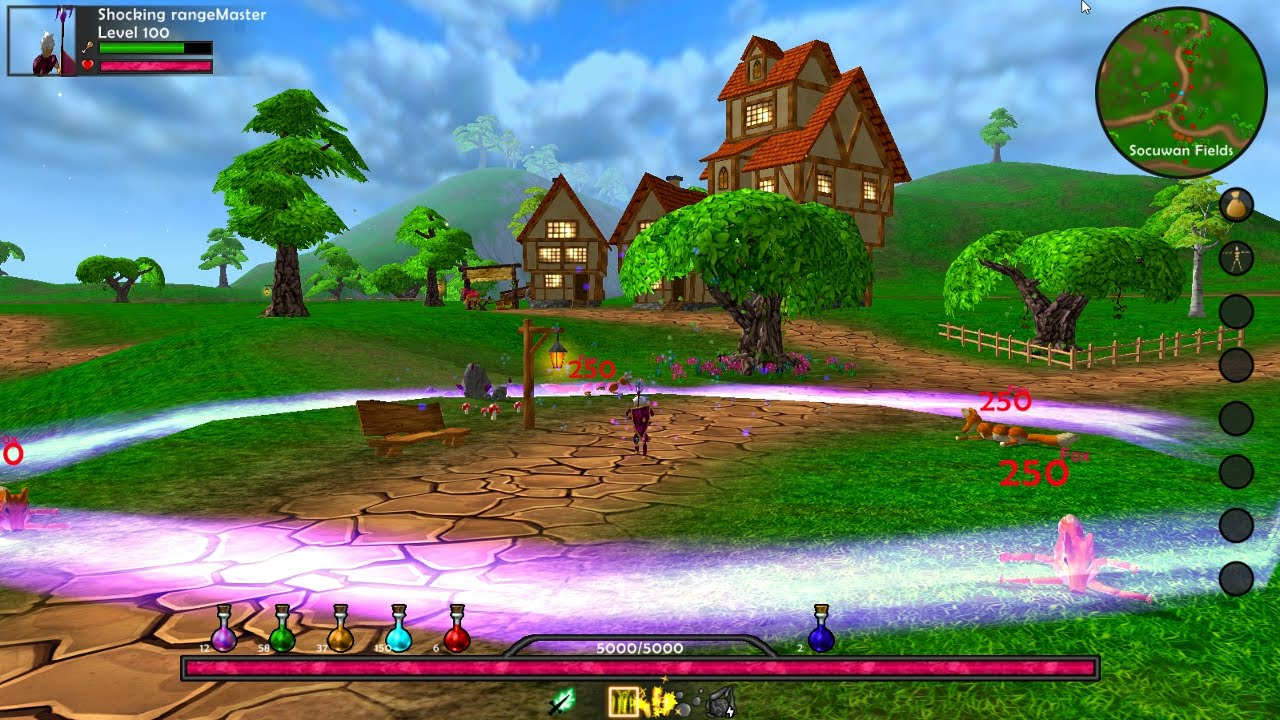
\includegraphics[width=1\linewidth, height = 200pt]{images/3dgame}
		\caption[Beispiel eines 3D Spiels]{Ausschnitt eines 3D Spiels in Java von ThinMatrix \cite{Fig2}}
	
\end{figure}

\clearpage

\section{Funktionsweise und Auswahl von Game Engines}\label{sec:jMonkeyEngine}
Um nicht sämtliche mathematischen Berechnungen auf der Grafikkarte selber programmieren, oder beispielsweise die Lautsprecher für Audio-Effekte ansprechen zu müssen, erhält der Entwickler Unterstützung durch sogenannte "Game Engines".
Diese beinhalten die Basisfunktionen von Spielen und ermöglichen dem Spiele-Programmierer eine gezieltere Entwicklung. Zu den Basisfunktionalitäten gehören im Allgemeinen die folgenden \cite{BF1}:
\begin{enumerate}
	\item Grafik-Engine
	\item Physiksystem
	\item Soundsystem
	\item Zustandsspeicherung
	\item Steuerung
	\item Datenverwaltung
\end{enumerate}
Zur Auswahl stehen eine Vielzahl von verschiedenen Engines, welche jeweils vor und Nachteile mit sich bringen. Da wir auf jeden Fall lernen wollten, wie die grundlegenden Dinge funktionieren, haben wir nach Engines gesucht, welche nur die Basisfunktionalitäten unterstützen, jedoch keine automatische Codegenerierung, Drag and Drop oder Editoren beinhalten.
Im folgenden eine Übersicht einiger Engines:


\begin{table}[h!]
	\myfloatalign
	\begin{tabularx}{\textwidth}{Xll} \toprule
		\tableheadline{GameEngine} & \tableheadline{Vorteile} & \tableheadline{Nachteile} \\ \midrule 
		Unity & Viele Benutzer, beliebt &  zu oberflächlich, kein Java \\
		jMonkeyEngine & Sehr entwicklungsnahe, Java & Schlechte Dokumentation \\
		Wurfel Engine & Benutzerfreundlich & Keine Physikunterstützung \\
		Cry Engine & Sehr schöne Grafik & Kein Java \\
		\bottomrule
	\end{tabularx}
	\caption[Engines]{Vor - und Nachteile einiger Game Engines \cite{GE1}}  \label{tab:example}
\end{table} 
Letztendlich fiel die Entscheidung auf die jMonkeyEngine, welche häufig von Java Entwicklern verwendet wird. 


\subsection {Die jMonkeyEngine}
Die jMonkeyEngine (jME) ist komplett in Java geschrieben und basiert auf dem Buch "3D Game Engine Design" von David Eberly \cite{GE2}.
Durch eine Abstraktionsschicht kann jedes beliebige Rendering System verwendet werden, beispielsweise die Lightweight Java Game Library (LWJGL) oder die Open Graphics Library (OpenGL).
Die neuste Version ist jME3, welche einige hilfreiche Funktionen mit sich bringt, wie beispielsweise ein Partikelsystem, Frustum Culling oder 3D Sound Unterstützung \cite{JM1}.
\begin{description}
	\item[Frustum Culling:] "Frustum Culling ist eine Optimierungsmethode, bei der all die Objekte vom Zeichnen ausgeschlossen werden, die außerhalb des Sichtbereichs (des Frustums) liegen." \cite{FC1}
\end{description}


\section{Umsetzung in Programmcode}\label{sec:code}
Im folgenden wird beschrieben wie einzelne Elemente in der jMonkeyEngine programmiert werden können und was dabei zu beachten ist. Die Erklärungen orientieren sich hierbei an dem jme3 Online-Beginners-Guide \cite{BG1} und der entsprechenden Dokumentation.

\subsection{Erzeugung der Application-Klasse: SimpleApplication}
Die Main-Klasse jedes jME3 Spieles erbt von der Klasse SimpleApplication, welche ein Spiel darstellt.
In der main-Methode wird dann eine neue Instanz erstellt und anschließend gestartet.

Jede Unterklasse der SimpleApplication beinhaltet die folgenden Methoden:
\begin{enumerate}
	\item simpleInitApp():
	Sorgt für das Laden von Modellen, der Erstellung einer räumlichen Umgebung sowie jegliche Initiierungen.
	\item simpleUpdate(float tpf):
	Wird für jedes frame per second (fps) ausgeführt und kümmert sich um gegebenenfalls geänderte Spielzustände.
	\item simpleRender(RenderManager rm):
	Wird stets nach simpleUpdate aufgerufen und zeichnet das Sichtbild des Spielers neu. Dazu bekommt die Methode einen RenderManager übergeben, welcher Präferenzen beim Zeichnen berücksichtigt (z.B. welche Ebene vorne oder hinten gezeichnet werden soll).
\end{enumerate} Die erste der drei Methoden wird stets zu Beginn ausgeführt um alle benötigten Elemente bereit zu stellen.

\subsection{Funktionsweise von Nodes}
Um Elemente zum Renderingprozess hinzuzufügen, um sie also sichtbar zu machen, müssen diese an ensprechende "Nodes" (engl. Knoten) angehängt werden.
Hierbei gibt es je nach Verwendungszweck verschiedene Arten zum Beispiel die \emph{audioNode} für Soundobjekte oder die \emph{guiNode} für Elemente auf der Benutzeroberfläche.\\
Final werden alle Nodes an die rootNode, also die Wurzel, angehängt. Im  Programmcode funktioniert dies mit der Methode \emph{attachChild()} bzw. \emph{detachChild()} zum entfernen.\\
Selbstverständlich können Objekte auch direkt an die rootNode angehängt werden, weshalb die Methodenparameter Modelle, Nodes, Bilder aber auch beispielsweise Audio-Files sind.
Allerdings ist es empfehlenswert eine geeignete Baumstruktur zu erstellen um so bestimmte Elemente in Gruppen anzusprechen.\\ \underline{\smash{Beispiel:}} Erzeugung einer eigenen Node durch:
\begin{lstlisting}
Node myNode = new Node();
myNode.doSomething();
\end{lstlisting}
Wird nun beispielsweise die folgende Funktion auf dem Konten ausgeführt, so wird diese auch für sämtliche Kinder des Knotens ausgeführt.





\subsection{Modelle und Assets}
Sämtliche externe Gegenstände des Spiels werden im \emph{assets}-Ordner im jME3 Projekt gesammelt. Dies sind multi-media Dateien wie 3D-Modelle, Soundfiles, Texturen, Shader und was sonst noch benötigt wird.
Um diese aus dem Ordner ins Spiel zu laden wird der sogenannte \emph{AssetManager} benötigt, welcher einfach eine Instanz der Klasse mit entsprechenden Funktionalitäten ist. \\Modelle sind dreidimensionale Gebilde welche verschiedenste Elemente in einem Spiel sein können. Hierbei verwendet jME3 die Klasse Spatial (engl. für "räumlich"). \\Zum Laden eines Objektes wird die entsprechende Funktion \emph{loadTexture(String path)} bzw. \emph{loadModel(String path)} aufgerufen und der entsprechende Pfad zum Modell übergeben:
\begin{center}
\fcolorbox{grau}{white}
{Spatial baum = assetManager.loadTexture("Models/Baum.j3o");}
\end{center} Für Modelle gibt es viele verschiedene Datentypen. Neben dem jMonkey-eigenen Dateiformat .j3o existieren einige weitere. Selbstverständlich ist meist eine Konversion zwischen den Formaten möglich. Die häufigsten von uns angetroffenen Vertreter für Modell-Deklarationen sind die folgenden:
\begin{enumerate}
	\item XML-Dateien: Aus einer mesh.xml Datei wird ein Objekt erzeugt. 
	\item OBJ-Dateien: Ein von \emph{Wavefront Technologies} entwickeltes Dateiformat für geometrische Formen. \cite{OBJ1}
	\item Blender-Dateien: Dies sind Dateien aus der Blender-Software, mit welcher Modelle erzeugt werden können.
\end{enumerate} Wie bereits unter \emph{Funktionsweise von Nodes} beschrieben müssen die Spatials nun lediglich zur rootNode, bzw. einer anderen Node welche mit der rootNode verknüpft ist, hinzugefügt werden. Damit werden die Modelle und Texturen sichtbar und sind Teil des Rendering-Prozesses.


\begin{center}
	\fcolorbox{grau}{white}
	{rootNode.attachChild(baum);}
\end{center} Der Aufbau von Modellen erfolgt durch entsprechende Software mit Polygonzügen oder Punktwolken. Dies definiert die allgemeine Struktur von Objekten.\\
Neben dieser und dem Material (vgl. \emph{Materialien}) gibt es noch das Skelett. Dieses kann ebenfalls in einem entsprechenden Programm wie Blender erzeugt und daraus bestimmte Bewegungsabläufe in Spielen bestimmt werden.
Das Skelett ist notwendig für Animationen von Modellen wie beispielsweise Gehen, Springen oder Ähnlichem.\\
In unserem Progman-Spiel haben wir uns für eine First-Person Perspektive entschieden, wodurch keine Animationen für den Spieler notwendig waren. Darüber hinaus haben wir uns auf Grund des Zeitaufwandes gegen eine Implementierung eines Skeletts beim Progman entschieden. Dieser ist daher nur eine starre Figur.



\subsection{Materialien}
Da in Modell-Software vorerst nur die Form von Figuren bestimmt wird, muss anschließend noch die Farbe, die Oberflächenstruktur und das Lichtverhalten bestimmt werden. Dies funktioniert über sogenannte \emph{'materials'}.\\
Die Datei für das Material kann in jme3 mit der Endung .mtl identifiziert werden. Diese bildet die entsprechenden Farbwerte von Bilddateien auf das Modell ab. Als Farbgeber sind beispielsweise mat.jpg oder mat.png gängig. Darüber hinaus können durch eine \emph{bump-map} und \emph{normalen}-Formate die Struktur der Oberfläche sowie das Verhalten bei Lichteinstrahlung (bspw. spiegelnd / schattierend /...) festgelegt werden. \\ Mit diesen Werkzeugen können sehr detaillierte Modellgenerierungen erfolgen, die nahezu realitätsgetreu sind.



\begin{figure}[h!]
	\myfloatalign
	\subfloat[Modell ohne Material]
	{
	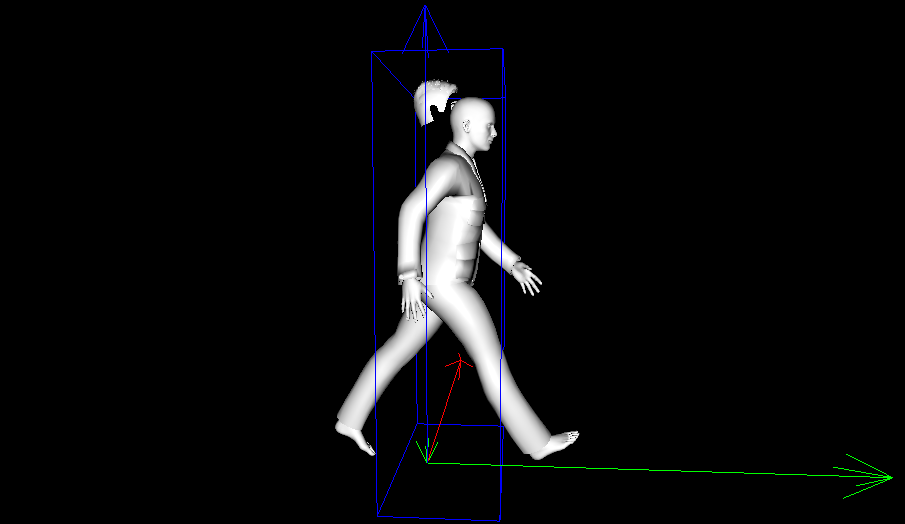
\includegraphics[width=.3\linewidth, height = 70pt]{images/modelmat}} \quad
	\subfloat[Modell mit Material]
	{\label{fig:example-b}%
	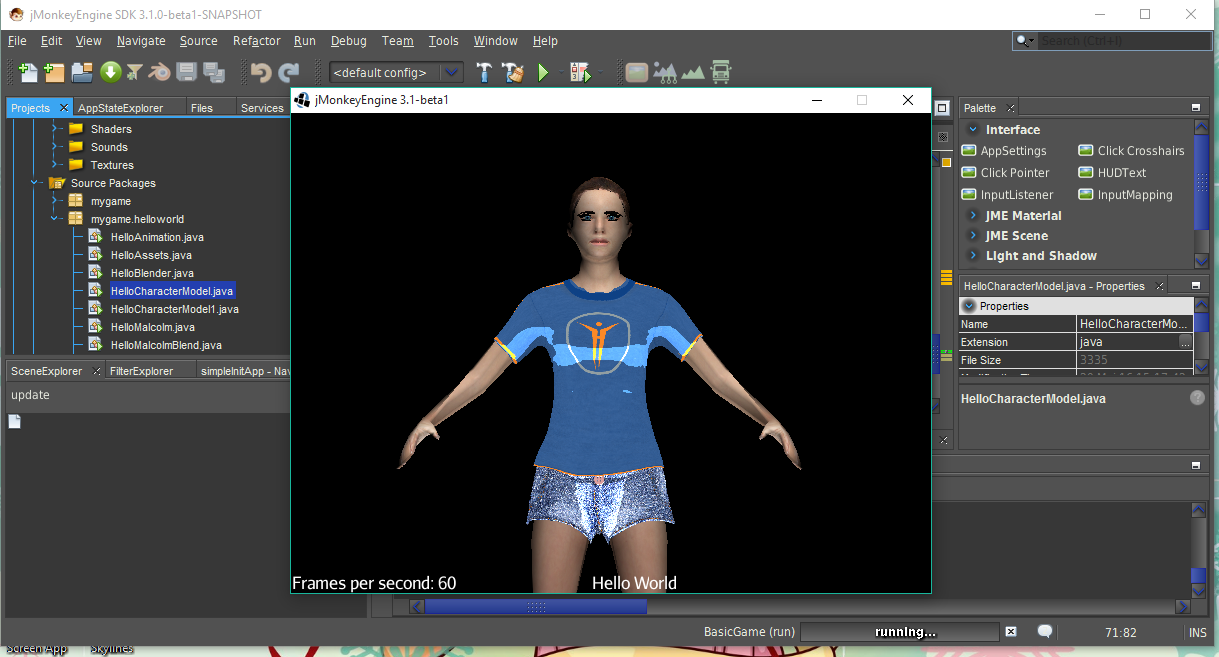
\includegraphics[width=.3\linewidth, height = 70pt]{images/modelmat2}} \\
	\caption[Materials auf Modellen]{Modell mit und ohne Material \cite{Fig1}}\label{fig:example}
	
\end{figure}







\subsection{User-Input}

Aus einem 3-dimensionalen Gebilde wird erst dann ein Spiel, wenn Interaktion mit dem Spieler stattfindet. Dazu müssen Tasteneingaben, Mauseingaben oder gegebenfalls auch Toucheingaben abgefangen und verarbeitet werden.
Hierbei werden die aus der ProkSy-Vorlesung bekannten Listener-Klassen verwendet.
Bezogen auf unser Spiel wurden folgende Aktionen durch Listener abgefangen:
\begin{enumerate}
	\item W/A/S/D: Dient zur Bewegung innerhalb des Spielraumes.
	\item Pfeiltasten/Maus: Zur Rundumsicht entsprechend einer Kopf-Bewegung.
	\item Taste "B": Aufnahme eines gefundenen Buches.
	\item Taste "L": Ein-/Ausschalten der Taschenlampe.
	\item Leertaste: Sprung
\end{enumerate} Zur Realisierung stehen in jme3 zwei wichtige Listener-Klassen zur Verfügung: Der \emph{ActionListener} und der \emph{AnalogListener}.
Ersterer sollte verwendet werden, wenn einzelne Aktionen erfolgen wie z.B. einmaliges Drücken der Taste B, zum Aufsammeln eines Buches.\\
Die zweite Klasse widerum, falls dauerhafte Events wie Gedrückthalten von W zur Vorwärtsbewegung abgefangen werden sollen. \\
Im Programmcode müssen dann entsprechende Aktionen erfolgen, damit der Input auch eine Auswirkung auf das Spiel hat. Beim Drücken von W müsste etwa der Richtungsvektor sowie die aktuelle Position abgefangen werden um eine Vorwärtsbewegung um x = walkingSpeed Richtungseinheiten zu erzeugen.

\subsection{Kollisionserkennung}
Damit man als Charakter nicht durch die gesamte Spielwelt gehen kann, müssen entsprechende Kollisionserkennungen eingebaut werden. So sollte der Spieler beispielsweise stoppen, wenn er sich in einen Baum hinein bewegen würde. Dazu kann in der Engine der folgende Code realisiert werden:


\begin{lstlisting}
CollisionShape shape = CollisionShapeFactor.createMeshShape(treeShape);
baumControl = new RigidBodyControl(shape);
baum.addControl(baumControl);
\end{lstlisting} Im ersten Schritt wird eine Form erstellt, welche das Modell annähert oder teilweise sogar mit ihm übereinstimmt. Bei Bäumen reichen theoretisch auch einfache Zylinder, da man mit der Baumkrone im Spiel sowieso nicht in Kontakt kommt. Im obigen Beispiel wird allerdings auf das Mesh, d.h  die tatsächliche Form zurückgegriffen.\\
Danach wir ein Art 'Überwacher' instantiiert, welcher sich um die Kollisionsfunktionalität kümmert. Dieser "kontrolliert" wann sich Modelle überlappen und verhindert dadurch ein Bewegen durch diese. Optional kann als Parameter auch die physikalische Masse des Objekts übergeben werden.\\
Im letzten Schritt wird dieser Control zum gewünschten Objekt hinzugefügt, damit eine entsprechende Kollisionserkennung stattfinden kann.\\
Bei Erzeugung einer Spielumgebung im \emph{SceneComposer} werden die physikalischen Eigenschaften bereits implizit implementiert.


\subsection{Erzeugung einer Spielumgebung}
Terrain oder SceneComposer, sky, 
Funktionalität und allgemeines vorgehen.
Wichtig: Beschreibung von Licht nicht vergessen (sonst dunkel)

\subsection{Hinzufügen von Audio}
Bei großen rollen-basierten Spielen erzeugen die Sound-Effekte, neben den grafischen Eigenschaften, den Hauptbestandteil der entsprechenden Atmosphäre. In unserem Spiel wurden folgende Sound-Effekte verwendet:
\begin{enumerate}
	\item Horror-Theme Soundtrack als Hintergrundmusik
	\item Donner-und Regensounds, welche zufällig abgespielt werden
	\item Fußstapfen im Wald
	\item Spezial Effekte wie beispielsweise: Knisterndes Feuer, Wolfs-Heulen, Spieler-Atmen, Herzklopfen...
\end{enumerate} Um Audio dem Spiel hinzuzufügen sind beispielhaft die folgenden Code-Zeilen notwendig (bei bereits existierender Instanz-Variable).

\begin{lstlisting}
audio_nature = new AudioNode(assetManager,"Sound/nature.mp3", true); // Laden
audio_nature.setLooping(true);  // Aktiviere wiederholendes Abspielen
audio_nature.setPositional(true); // Raeumliche Audio-Effekte  
audio_nature.setVolume(3); // Lautstaerke festlegen
rootNode.attachChild(audio_nature); 
audio_nature.play(); // Abspielen des Sounds
\end{lstlisting}


\subsection{Physikalische Modellierung}
Die jme3 Engine erlaubt durch ihre Physik-Engine Objekten verschiedenes physikalisches Verhalten zuzuordnen. Die Kräfte, welche wirken sind dann je nach Masse verschieden.\\
In unserem Spiel haben wir hauptsächlich von der Schwerkraft Gebrauch gemacht, welche sich durch den Befehl\emph{ setGravity()} auf Spatials anwenden lässt.

\subsection{Effekte und Details}
Um dem Spiel mehr Leben einzuhauchen können verschiedenste Spezialeffekte erstellt werden. Im Folgenden wird auf zwei wichtige Beispiele eingegangen und wie diese in der jMonkeyEngine umgesetzt werden können.
\subsubsection{Nebel}
In unserem Wald haben wir zur besseren Atmosphäre einen Nebeleffekt hinzugefügt. Genaugenommen ist dies lediglich eine Erhellung der Pixel in Abhängigkeit des Abstandes vom Spieler. Es gibt zwei Möglichkeiten im Code Nebel zu erzeugen:
\begin{enumerate}
	\item[1.] Programieren eines Shaders 
	\item[2.] Verwendung des FogFilters in jme3
\end{enumerate}
Da wir uns für die Theorie dahinter interessierten haben wir uns über das allgemeine Vorgehen für 1. informiert aber letztendlich den FogFilter verwendet.
Die Berechnung des Nebels erfolgt exponentiell mit Berücksichtigung von Lichteffekten, abhängig vom Abstand zum Spieler. Entsprechende Erklärungen können unter \cite{Cr14} nachgeschlagen werden.

\begin{equation}
	FinalFogColor = (1.0-e^{db\textrm{1}})*fogColor + e^{db\textrm{2}} * lightColor \\
\end{equation} Wobei \\ \emph{
	d = Abstand zum Spieler} \\
	\emph{b = Nebeldichte je nach Lichteffekt} sind.


\begin{figure}[h!]
	\myfloatalign
	\caption{Exponentieller Nebel - Ergebnis}
	
	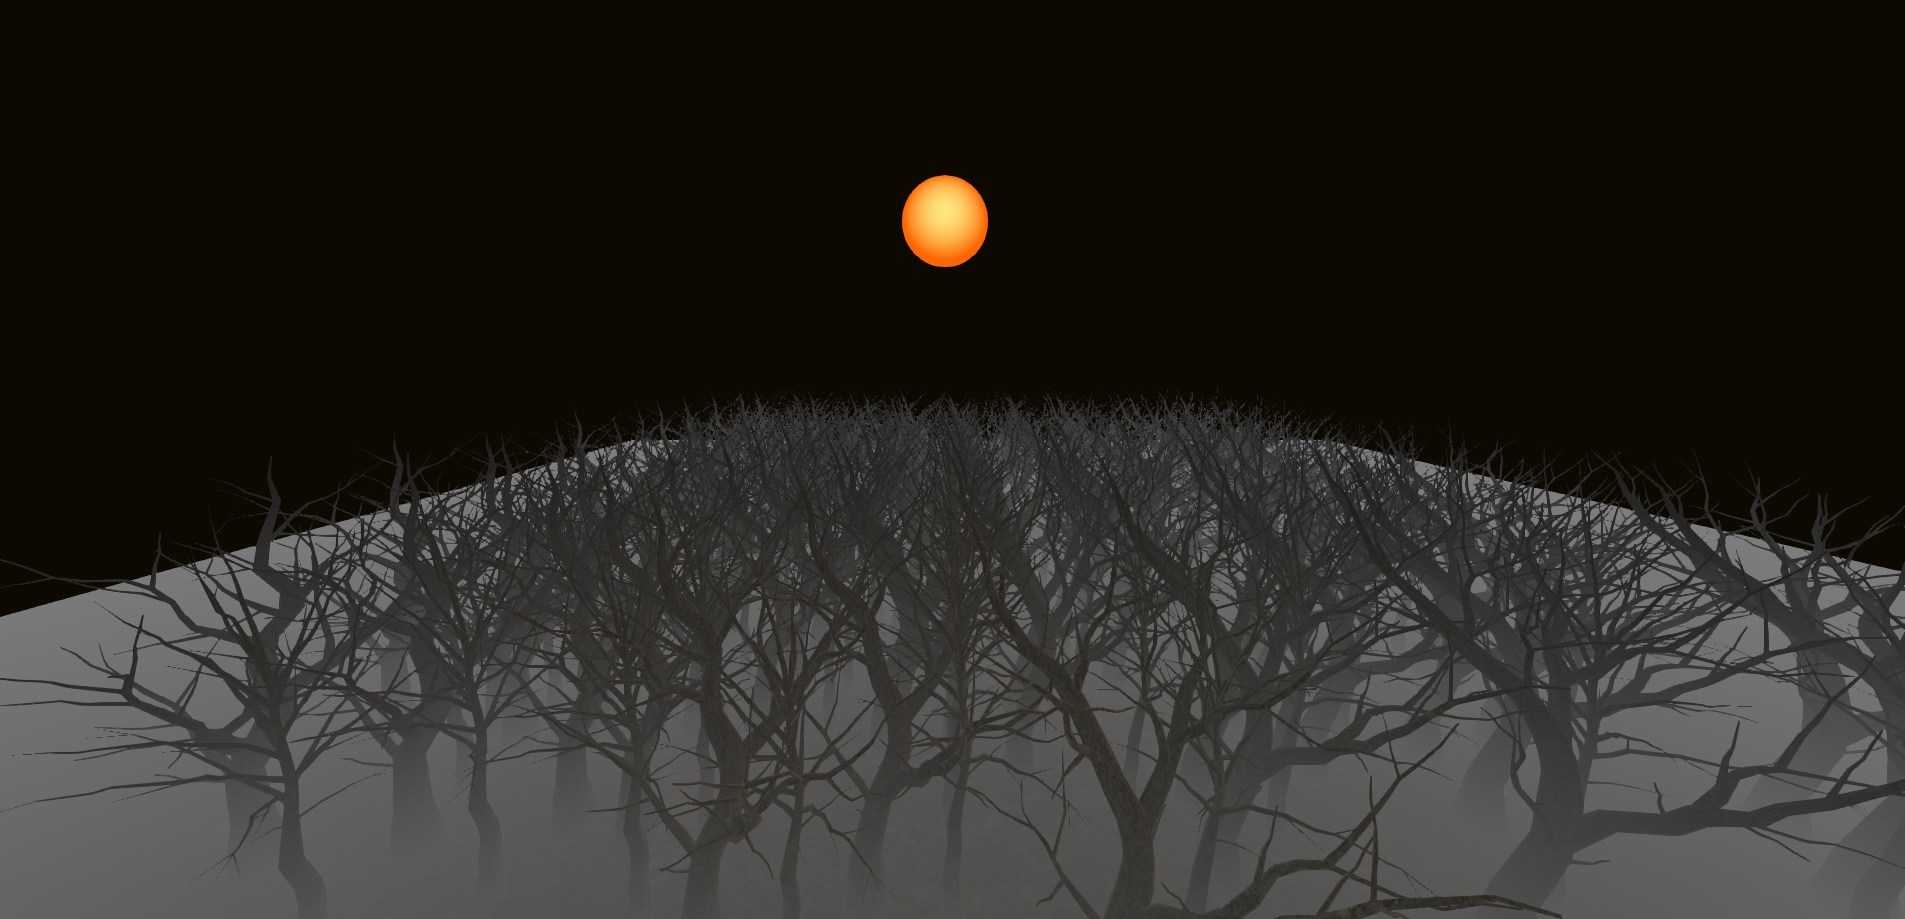
\includegraphics[width=.9\linewidth, height = 200pt]{images/fog} 
	
\end{figure}

\subsubsection{Partikeleffekte}
In fast jeder 3D-Game-Engine existieren Partikeleffekte. Dabei werden Partikel verschiedenster Formen und Größen mit unterschiedlichen Geschwindigkeiten in den Raum gezeichnet. Dadurch lassen sich beispielsweise Effekte wie ein brennendes Feuer, Schnee, Regen oder Explosionen erstellen. In jme3 existiert hierfür die Klasse \emph{ParticleEmitter}, welche sich um das Verhalten der Partikel kümmert.\\
In unserem Progman-Spiel kam diese in zwei Fällen zur Anwendung: Leichter Regen, sowie ein kleines Feuerchen in der nähe eines Hauses.\\ Im Folgenden ein Code-Beispiel wie Partikeleffekte erzeugt werden können, sowie Ausschnitte aus unserem Spiel.

\begin{lstlisting}
ParticleEmitter pm = new ParticleEmitter("effect", Type.Triangle, 60);
Material pmMat = new Material(assetManager, "Common/MatDefs/Misc/Particle.j3md");
pmMat.setTexture("Texture", assetManager.loadTexture("Effects/rain.png"));
pm.setMaterial(pmMat);
pm.setImagesX(1);
pm.setImagesY(1);
rootNode.attachChild(pm);
\end{lstlisting}


\section{Optimierung des Programms}\label{sec:optimizing}
Wenn man wie oben beschrieben einige Modelle und Effekte in seine Spielumgebung einbindet, können der Prozessor bzw. die Grafikkarte sehr schnell an Grenzen stoßen. Dabei spielt die Anzahl der Vertexes bzw. Triangles eine zentrale Rolle. Jedes Modell hat unter Umständen einige tausend Triangles, sodass sich dies in einem Spiel sehr leicht aufsummieren kann. In unserem Spiel gibt es zum Beispiel knapp 2000 Bäume, welche alle gerendert werden müssen: Vereinfacht man dort das Modell des Baumes, hat dies viel Potenzial, das gesamte Spiel zu beschleunigen. Mit Hilfe von \emph{F5} kann man in jMonkey während des Spiels anzeigen lassen, wie viele Triangles und Vertexes gerade zu rendern sind. Es versteht sich von selbst, dass ein Spiel mit einigen Millionen Vertexes viel zu aufwendig wird, weshalb die Framerate meist auf nahezu null sinkt. Um dies zu verhindern, muss man also die Anzahl an Triangles und Vertexes verringern. Dies ist grundsätzlich durch die Minimierung der Anzahl von Modellen oder durch die Minimierung der Anzahl an Triangles und Vertexes innerhalb eines Modells möglich. Diese haben dafür oft ein sogenanntes LevelOfDetail (kurz LOD), welches abhängig von der Nähe Texturen und Modelle immer genauer zeichnet.

Interessanterweise fiel uns auf, dass das Terrain selbst (also der Untergrund des Spielers) sehr viele Triangles besitzt. Das liegt daran, dass das Terrain dafür ausgelegt ist aufwendige Umgebungen darzustellen (sog. \emph{heightmaps}). So können Gebirge oder sonstige Unebenheiten sehr fein erstellt werden. Der Nachteil dabei ist jedoch, dass es sehr aufwendig wird das Terrain selbst ohne Models zu rendern, obwohl diese wie in unserem Beispiel einfach nur gerade sein kann. Es ist also unbedingt notwendig bei der Programmierung eines 3D-Spiels auf die Framerate und Komplexität der Welt zu achten.



\subsubsection{Minimierung der Anzahl von Modellen}
Um eine hohe Spielgeschwindigkeit zu gewährleisten bietet sich vorerst an, das Spiel möglichst simpel zu halten. Dies kann zum Beispiel erreicht werden, indem die Anzahl der benutzten Modelle reduziert wird. Also sollte man keine unnötigen Modelle verwenden, die nicht gebraucht werden. Man könnte zum Beispiel Modelle, welche von der Kameraposition im Spiel weit entfernt sind ausblenden, da diese sowieso nicht gesehen werden. In jMonkey kann man die Distanz einstellen, ab welcher die Modelle nicht mehr gerendert werden. Hier ein Beispiel aus unserem Code


\begin{lstlisting}
camera.setFrustumPerspective(45f, (float)cam.getWidth() / cam.getHeight(),1f,400f); //nur bis 100 Meter
\end{lstlisting}


Somit muss in unserem Beispiel nicht jeder der fast 2000 Bäume gerendert werden, sondern nur in der Nähe des Spielers. Auf diesem Weg kann sehr einfach die Komplexität der darzustellenden Welt reduziert werden.

\subsubsection{Level of Detail (LOD)}
In der jMonkeyEngine ist es grundsätzlich vorgesehen, dass man seinen Modellen eigene LODs gibt. Damit kann man anhand dieser LODs die Komplexität des Models im Laufe des Spiels bzw. vor dem Spiel verändern. Dabei gilt es noch zu beachten, dass die Modelle selbst keine LODs haben, sondern die Geometries, welchen sie zugrunde liegen. Man kann innerhalb des SceneExplorers die einzelnen Modelle und deren Geometries auswählen, und eigene LODs generieren:\\
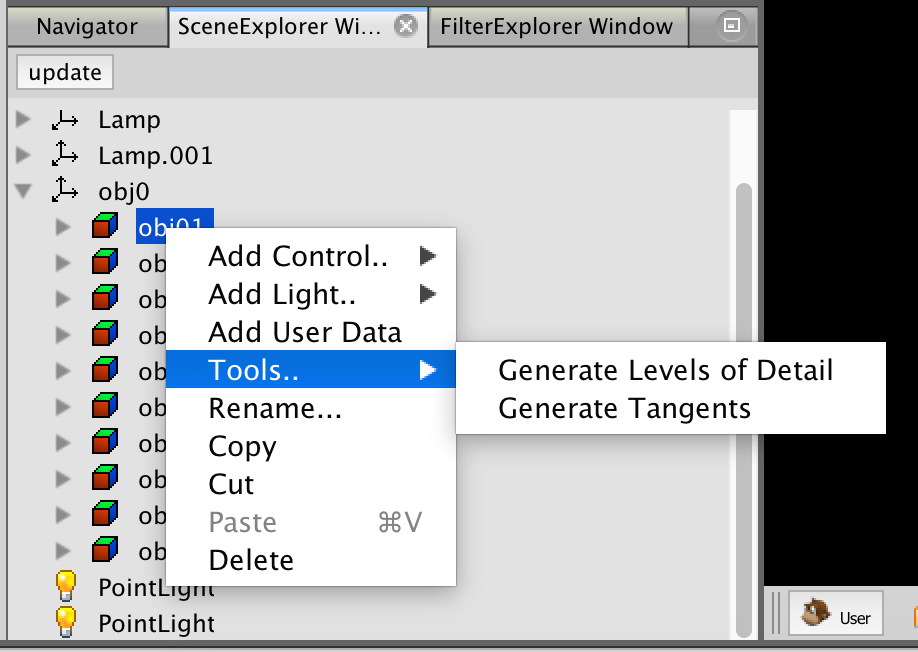
\includegraphics[width=1\linewidth]{images/generateLOD.png}



Ein alternativer Weg ist, dass man der Geometry eines vorhandenen Spatials während der Laufzeit einen neuen LOD-Wert zuweist. 

\section{Kritik an der jMonkeyEngine3}



\appendix % ab hier folgt der Anhang
%********************************************************************
% Appendix
%*******************************************************
\chapter{Anhang A}




%********************************************************************
% Other Stuff in the Back
%*******************************************************
%\cleardoublepage%********************************************************************
% Bibliography
%*******************************************************
% work-around to have small caps also here in the headline
\manualmark
\markboth{\spacedlowsmallcaps{\bibname}}{\spacedlowsmallcaps{\bibname}} % work-around to have small caps also
%\phantomsection 
\refstepcounter{dummy}
\addtocontents{toc}{\protect\vspace{\beforebibskip}} % to have the bib a bit from the rest in the toc
\addcontentsline{toc}{chapter}{\tocEntry{\bibname}}
\label{app:bibliography}
%\printbibliography
%\bibliographystyle{../lnig}
%\bibliography{bibliography}
%\bibliographystyle{geralpha} %Literaturverzeichnis
% \bibliography{Bibliography} %Literaturverzeichnis

%********************************************************************
% Bibliography
%*******************************************************
% work-around to have small caps also here in the headline
\manualmark
\markboth{\spacedlowsmallcaps{\bibname}}{\spacedlowsmallcaps{\bibname}} % work-around to have small caps also
%\phantomsection 
\refstepcounter{dummy}
\addtocontents{toc}{\protect\vspace{\beforebibskip}} % to have the bib a bit from the rest in the toc
\addcontentsline{toc}{chapter}{\tocEntry{\bibname}}
\label{app:bibliography}
\bibliographystyle{lnig}
%\bibliographystyle{itmabbrv}
\bibliography{bibliography}
\cleardoublepage%*******************************************************
% Declaration
%*******************************************************
\refstepcounter{dummy}
\pdfbookmark[0]{Erklärung}{erklärung}
\chapter*{Erklärung}
\thispagestyle{empty}



\bigskip
 
\noindent\textit{\myLocation, \myTime}

\smallskip

\begin{flushright}
    \begin{tabular}{m{8cm}}
        \\ \hline
        \centering\myName \\
    \end{tabular}
\end{flushright}



% ********************************************************************
%*******************************************************
\end{document}
% ********************************************************************
